% Created by tikzDevice version 0.12.3.1 on 2021-10-17 10:40:52
% !TEX encoding = UTF-8 Unicode
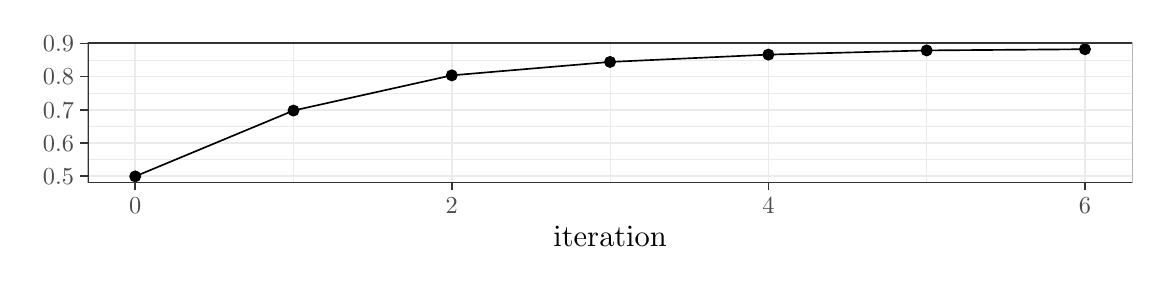
\begin{tikzpicture}[x=1pt,y=1pt]
\definecolor{fillColor}{RGB}{255,255,255}
\path[use as bounding box,fill=fillColor,fill opacity=0.00] (0,0) rectangle (404.71, 86.72);
\begin{scope}
\path[clip] (  0.00,  0.00) rectangle (404.71, 86.72);
\definecolor{drawColor}{RGB}{255,255,255}
\definecolor{fillColor}{RGB}{255,255,255}

\path[draw=drawColor,line width= 0.6pt,line join=round,line cap=round,fill=fillColor] (  0.00,  0.00) rectangle (404.71, 86.72);
\end{scope}
\begin{scope}
\path[clip] ( 21.69, 30.69) rectangle (399.21, 81.22);
\definecolor{fillColor}{RGB}{255,255,255}

\path[fill=fillColor] ( 21.69, 30.69) rectangle (399.21, 81.22);
\definecolor{drawColor}{gray}{0.92}

\path[draw=drawColor,line width= 0.3pt,line join=round] ( 21.69, 39.04) --
	(399.21, 39.04);

\path[draw=drawColor,line width= 0.3pt,line join=round] ( 21.69, 51.04) --
	(399.21, 51.04);

\path[draw=drawColor,line width= 0.3pt,line join=round] ( 21.69, 63.04) --
	(399.21, 63.04);

\path[draw=drawColor,line width= 0.3pt,line join=round] ( 21.69, 75.04) --
	(399.21, 75.04);

\path[draw=drawColor,line width= 0.3pt,line join=round] ( 96.05, 30.69) --
	( 96.05, 81.22);

\path[draw=drawColor,line width= 0.3pt,line join=round] (210.45, 30.69) --
	(210.45, 81.22);

\path[draw=drawColor,line width= 0.3pt,line join=round] (324.85, 30.69) --
	(324.85, 81.22);

\path[draw=drawColor,line width= 0.6pt,line join=round] ( 21.69, 33.04) --
	(399.21, 33.04);

\path[draw=drawColor,line width= 0.6pt,line join=round] ( 21.69, 45.04) --
	(399.21, 45.04);

\path[draw=drawColor,line width= 0.6pt,line join=round] ( 21.69, 57.04) --
	(399.21, 57.04);

\path[draw=drawColor,line width= 0.6pt,line join=round] ( 21.69, 69.04) --
	(399.21, 69.04);

\path[draw=drawColor,line width= 0.6pt,line join=round] ( 21.69, 81.04) --
	(399.21, 81.04);

\path[draw=drawColor,line width= 0.6pt,line join=round] ( 38.85, 30.69) --
	( 38.85, 81.22);

\path[draw=drawColor,line width= 0.6pt,line join=round] (153.25, 30.69) --
	(153.25, 81.22);

\path[draw=drawColor,line width= 0.6pt,line join=round] (267.65, 30.69) --
	(267.65, 81.22);

\path[draw=drawColor,line width= 0.6pt,line join=round] (382.05, 30.69) --
	(382.05, 81.22);
\definecolor{drawColor}{RGB}{0,0,0}

\path[draw=drawColor,line width= 0.6pt,line join=round] ( 38.85, 32.98) --
	( 96.05, 56.77) --
	(153.25, 69.49) --
	(210.45, 74.34) --
	(267.65, 76.98) --
	(324.85, 78.50) --
	(382.05, 78.93);
\definecolor{fillColor}{RGB}{0,0,0}

\path[draw=drawColor,line width= 0.4pt,line join=round,line cap=round,fill=fillColor] ( 38.85, 32.98) circle (  1.96);

\path[draw=drawColor,line width= 0.4pt,line join=round,line cap=round,fill=fillColor] ( 96.05, 56.77) circle (  1.96);

\path[draw=drawColor,line width= 0.4pt,line join=round,line cap=round,fill=fillColor] (153.25, 69.49) circle (  1.96);

\path[draw=drawColor,line width= 0.4pt,line join=round,line cap=round,fill=fillColor] (210.45, 74.34) circle (  1.96);

\path[draw=drawColor,line width= 0.4pt,line join=round,line cap=round,fill=fillColor] (267.65, 76.98) circle (  1.96);

\path[draw=drawColor,line width= 0.4pt,line join=round,line cap=round,fill=fillColor] (324.85, 78.50) circle (  1.96);

\path[draw=drawColor,line width= 0.4pt,line join=round,line cap=round,fill=fillColor] (382.05, 78.93) circle (  1.96);
\definecolor{drawColor}{gray}{0.20}

\path[draw=drawColor,line width= 0.6pt,line join=round,line cap=round] ( 21.69, 30.69) rectangle (399.21, 81.22);
\end{scope}
\begin{scope}
\path[clip] (  0.00,  0.00) rectangle (404.71, 86.72);
\definecolor{drawColor}{gray}{0.30}

\node[text=drawColor,anchor=base east,inner sep=0pt, outer sep=0pt, scale=  0.88] at ( 16.74, 30.01) {0.5};

\node[text=drawColor,anchor=base east,inner sep=0pt, outer sep=0pt, scale=  0.88] at ( 16.74, 42.01) {0.6};

\node[text=drawColor,anchor=base east,inner sep=0pt, outer sep=0pt, scale=  0.88] at ( 16.74, 54.01) {0.7};

\node[text=drawColor,anchor=base east,inner sep=0pt, outer sep=0pt, scale=  0.88] at ( 16.74, 66.01) {0.8};

\node[text=drawColor,anchor=base east,inner sep=0pt, outer sep=0pt, scale=  0.88] at ( 16.74, 78.01) {0.9};
\end{scope}
\begin{scope}
\path[clip] (  0.00,  0.00) rectangle (404.71, 86.72);
\definecolor{drawColor}{gray}{0.20}

\path[draw=drawColor,line width= 0.6pt,line join=round] ( 18.94, 33.04) --
	( 21.69, 33.04);

\path[draw=drawColor,line width= 0.6pt,line join=round] ( 18.94, 45.04) --
	( 21.69, 45.04);

\path[draw=drawColor,line width= 0.6pt,line join=round] ( 18.94, 57.04) --
	( 21.69, 57.04);

\path[draw=drawColor,line width= 0.6pt,line join=round] ( 18.94, 69.04) --
	( 21.69, 69.04);

\path[draw=drawColor,line width= 0.6pt,line join=round] ( 18.94, 81.04) --
	( 21.69, 81.04);
\end{scope}
\begin{scope}
\path[clip] (  0.00,  0.00) rectangle (404.71, 86.72);
\definecolor{drawColor}{gray}{0.20}

\path[draw=drawColor,line width= 0.6pt,line join=round] ( 38.85, 27.94) --
	( 38.85, 30.69);

\path[draw=drawColor,line width= 0.6pt,line join=round] (153.25, 27.94) --
	(153.25, 30.69);

\path[draw=drawColor,line width= 0.6pt,line join=round] (267.65, 27.94) --
	(267.65, 30.69);

\path[draw=drawColor,line width= 0.6pt,line join=round] (382.05, 27.94) --
	(382.05, 30.69);
\end{scope}
\begin{scope}
\path[clip] (  0.00,  0.00) rectangle (404.71, 86.72);
\definecolor{drawColor}{gray}{0.30}

\node[text=drawColor,anchor=base,inner sep=0pt, outer sep=0pt, scale=  0.88] at ( 38.85, 19.68) {0};

\node[text=drawColor,anchor=base,inner sep=0pt, outer sep=0pt, scale=  0.88] at (153.25, 19.68) {2};

\node[text=drawColor,anchor=base,inner sep=0pt, outer sep=0pt, scale=  0.88] at (267.65, 19.68) {4};

\node[text=drawColor,anchor=base,inner sep=0pt, outer sep=0pt, scale=  0.88] at (382.05, 19.68) {6};
\end{scope}
\begin{scope}
\path[clip] (  0.00,  0.00) rectangle (404.71, 86.72);
\definecolor{drawColor}{RGB}{0,0,0}

\node[text=drawColor,anchor=base,inner sep=0pt, outer sep=0pt, scale=  1.10] at (210.45,  7.64) {iteration};
\end{scope}
\end{tikzpicture}
